% ============================================================
% CHAPTER 7: RESULTS
% ============================================================

\chapter{Results}

Trustless Notes is a fully functional zero-knowledge encrypted note-taking application that demonstrates the practical application of modern web cryptography and network security principles. The system successfully implements client-side encryption using the Web Cryptography API, ensuring that the server never has access to plaintext user data.

% ------------------------------------------------------------
\section{Implemented Features}
% ------------------------------------------------------------

The following features have been successfully implemented:

\begin{itemize}
    \item \textbf{Zero-Knowledge Authentication:} Account creation and sign-in without transmitting the password. PBKDF2 key derivation with 200,000 iterations of SHA-256 produces non-extractable AES-256-GCM keys. Sentinel-based verification ensures the server cannot verify passwords or enumerate usernames.

    \item \textbf{Encrypted Note Management:} Create, read, update, and delete operations on notes, each encrypted with a unique AES-256-GCM key. Note keys are independently wrapped by the user's derived key. Debounced auto-save (800ms) provides a seamless editing experience.

    \item \textbf{Cryptographic Note Sharing:} ECDH P-256 key exchange with HKDF-derived symmetric keys enables secure note sharing. The server mediates the exchange but cannot decrypt the shared content.

    \item \textbf{Encrypted File Attachments:} Image files are encrypted client-side before upload to Supabase Storage. Decryption and display occur entirely in the browser, with decrypted data existing only as in-memory Blob URLs.

    \item \textbf{Signed Cookie Session Management:} HMAC-SHA256 signed cookies provide tamper-proof session state without exposing sensitive credentials.

    \item \textbf{Security Simulator:} Four interactive attack scenarios visually demonstrate the system's resistance to database leaks, password leaks, cookie forgery, and service key compromises.

    \item \textbf{Anti-Enumeration Sign-In:} The sign-in endpoint returns indistinguishable responses for valid and invalid usernames, preventing username enumeration attacks.
\end{itemize}

% ------------------------------------------------------------
\section{Application Screenshots}
% ------------------------------------------------------------

The following figures illustrate the user interface of the Trustless Notes application.

\begin{figure}[htbp]
    \centering

    % ---------- Row 1 ----------
    \begin{subfigure}{0.45\textwidth}
        \centering
        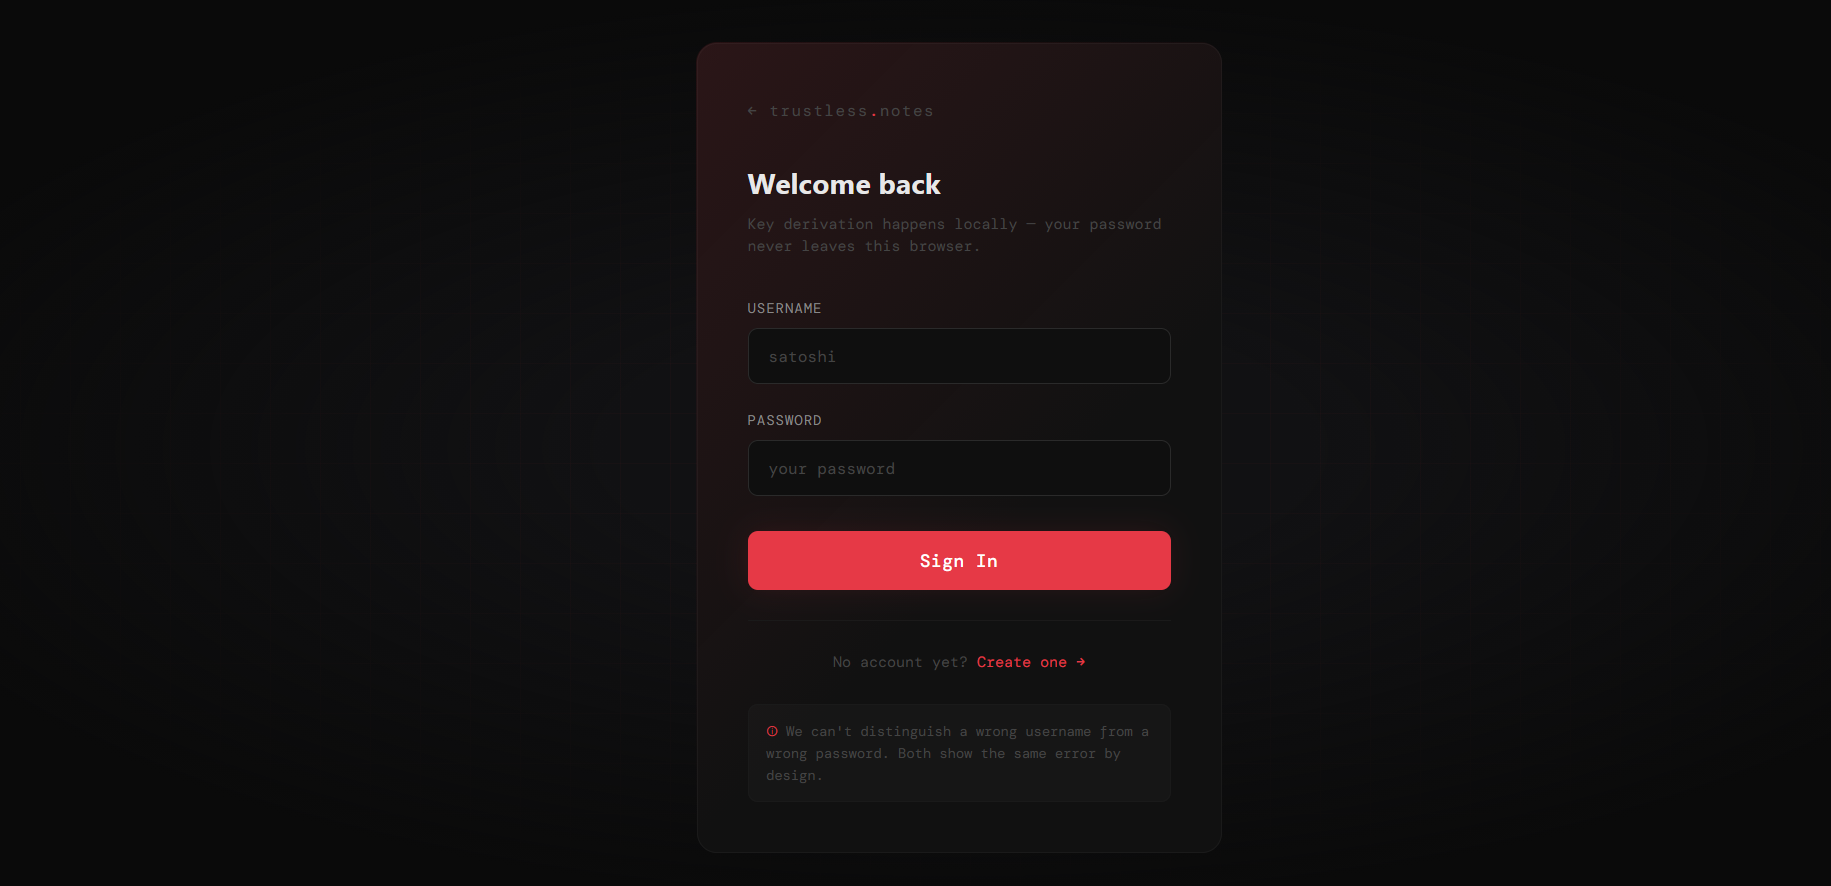
\includegraphics[width=\textwidth]{media/signin.png}
        \caption{Sign-In Page}
    \end{subfigure}
    \hfill
    \begin{subfigure}{0.45\textwidth}
        \centering
        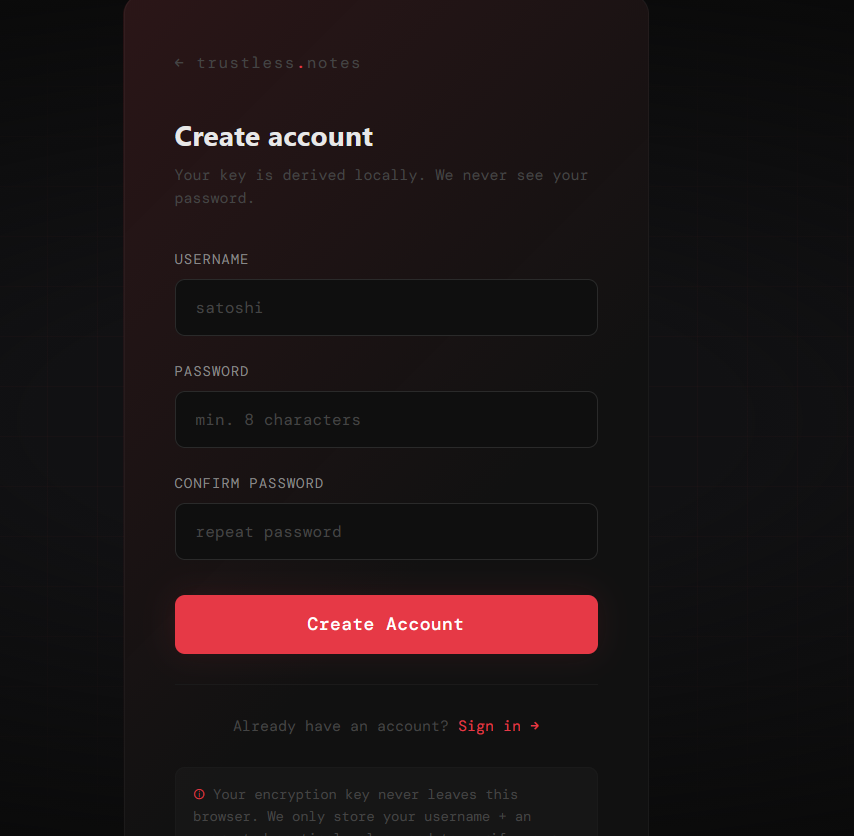
\includegraphics[width=\textwidth]{media/signup.png}
        \caption{Sign-Up Page}
    \end{subfigure}

    \vspace{0.6cm}

    % ---------- Row 2 ----------
    \begin{subfigure}{0.45\textwidth}
        \centering
        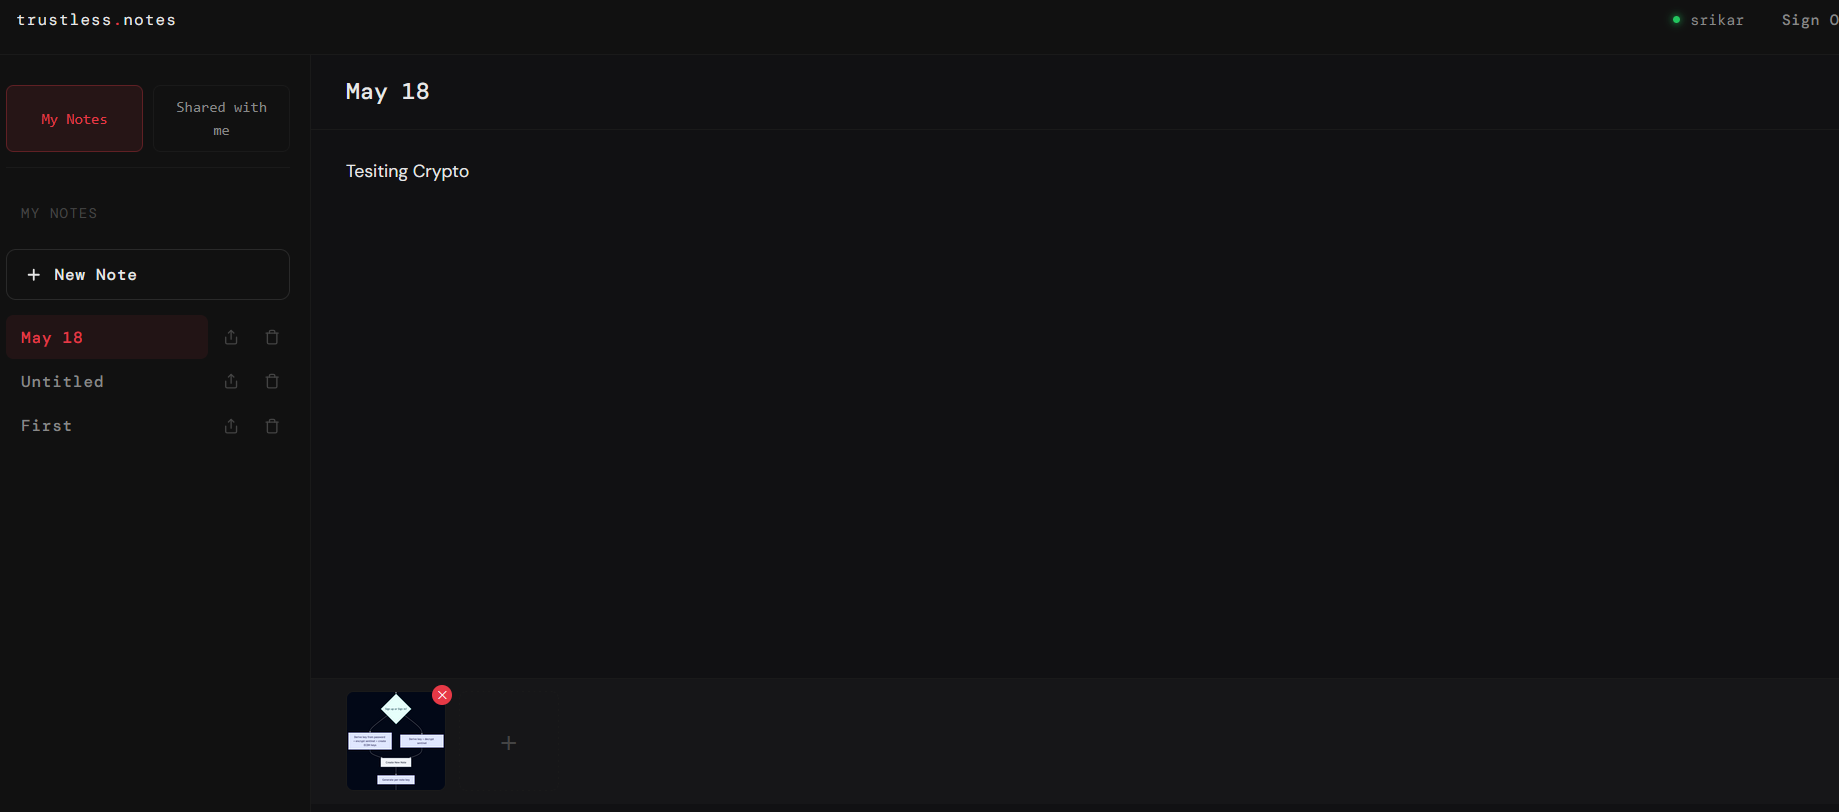
\includegraphics[width=\textwidth]{media/dashboard.png}
        \caption{Dashboard with Notes Sidebar}
    \end{subfigure}
    \hfill
    \begin{subfigure}{0.45\textwidth}
        \centering
        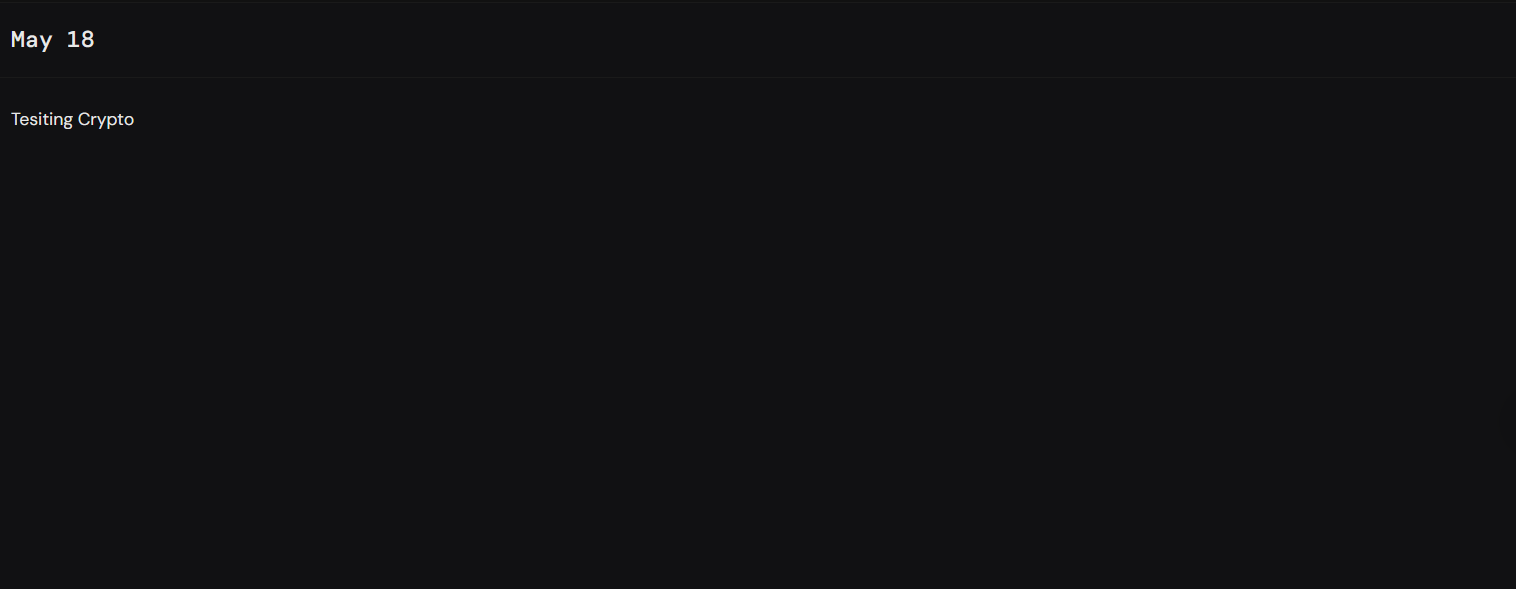
\includegraphics[width=\textwidth]{media/note-editor.png}
        \caption{Note Editor with Markdown Rendering}
    \end{subfigure}

    \vspace{0.6cm}

    % ---------- Row 3 ----------
    \begin{subfigure}{0.45\textwidth}
        \centering
        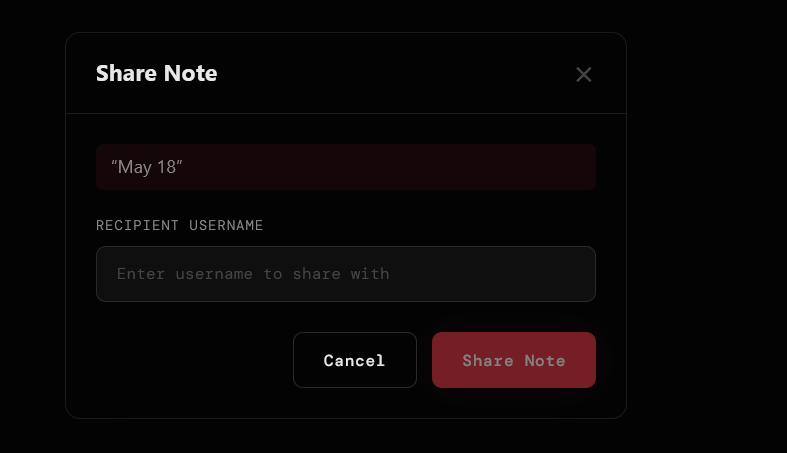
\includegraphics[width=\textwidth]{media/share-modal.png}
        \caption{Share Modal Interface}
    \end{subfigure}
    \hfill
    \begin{subfigure}{0.45\textwidth}
        \centering
        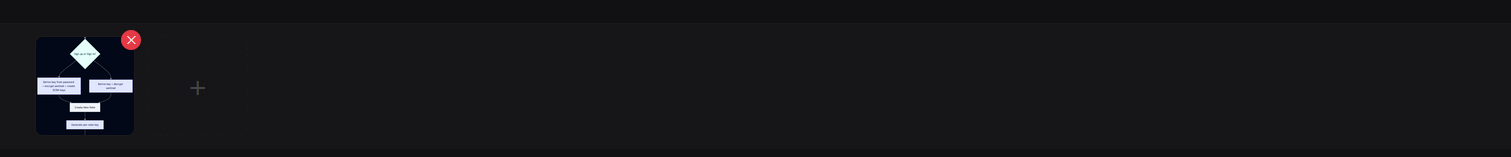
\includegraphics[width=\textwidth]{media/attachment-dock.png}
        \caption{Image Attachment Dock}
    \end{subfigure}

    \vspace{0.6cm}

    % ---------- Row 4 ----------
    \begin{subfigure}{0.65\textwidth}
        \centering
        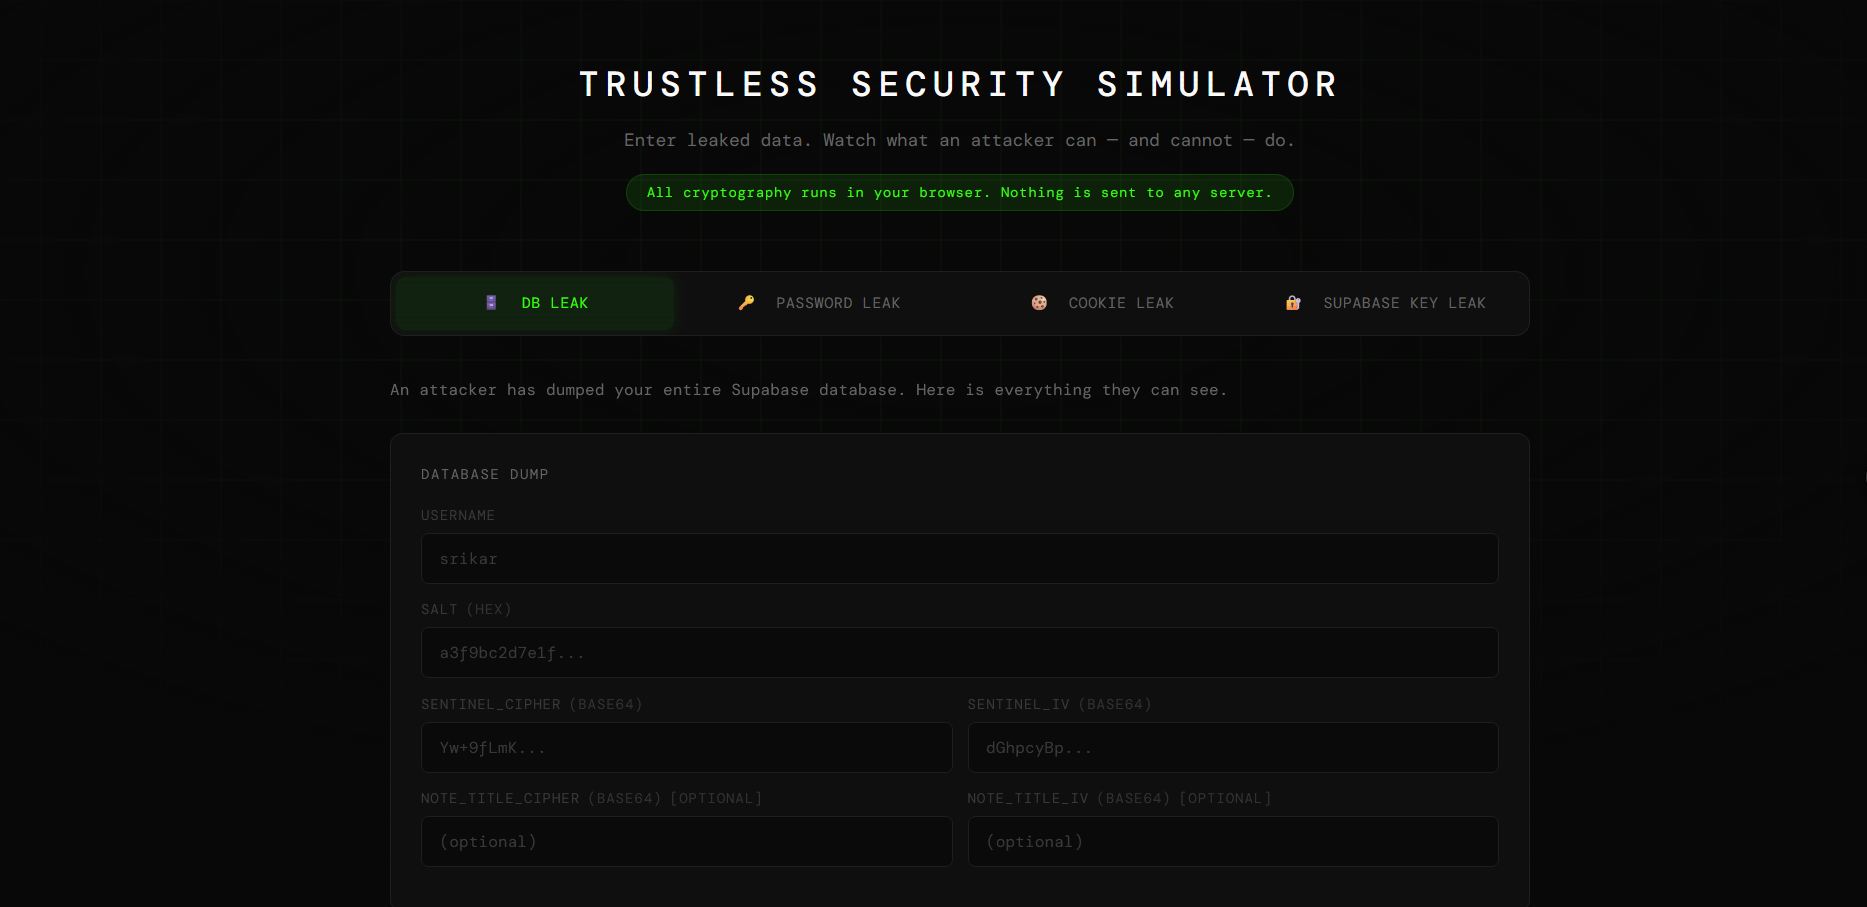
\includegraphics[width=\textwidth]{media/simulator-db-leak.png}
        \caption{Security Simulator}
    \end{subfigure}

    \caption{Trustless Notes Application Interfaces}
    \label{fig:ui_results}
\end{figure}
